
% Add "answers" option to print the answers
\documentclass[addpoints]{exam}

\usepackage[utf8]{inputenc}
\usepackage{calc}
\usepackage[dvipsnames]{xcolor}
\usepackage{ifthen}
\usepackage{tcolorbox}

% \makebox[\textwidth]{Name:\enspace\hrulefill}
%  
% \vspace{5mm}
%\makebox[\textwidth]{Instructor’s name:\enspace\hrulefill}

\definecolor{MyLightGray}{gray}{0.60}

\newcommand{\truefalse}
{		\begin{checkboxes}
			 \choice True
			 \choice False. Explanation: 
		\end{checkboxes}
		\vspace{10pt}
}


% Check if 'answers' is an option
\newcommand{\ifanswers}[2]{%
  \ifthenelse{\boolean{exam@answers}}{#1}{#2}%
}



\newcommand{\answerspace}[1]
{
	\ifprintanswers
	\else
		\setlength{\mylength}{10pt}%
		% \vspace{#1\mylength}
		% Make the grey box
		\par\nobreak\noindent
		\makebox[\linewidth][l]{%
			% set inner padding to zero, so only the frame shows
			{\setlength{\fboxsep}{0pt}%
			% draw a color frame, white (or transparent) inside
			\fcolorbox{MyLightGray}{white}{%
			% the inner box has zero width content but fixed height
			\parbox[t][#1\mylength][c]{%
				% subtract twice the frame‐thickness from the full width
				\dimexpr\linewidth-2\fboxrule\relax
			}{\strut}%
			}%
			}%
		}%
		\par
		\vspace{3\mylength}

  	\fi
}
\newlength{\mylength}

\newcommand{\code}[1]{{\texttt{#1}}}

\newcommand{\answer}[1]{\begin{solution}{#1}\end{solution}}




%\usepackage{listings}
\usepackage{color}
\usepackage{lastpage}
\usepackage{verbatim}
\usepackage{fancyvrb}
\usepackage{graphicx}
\usepackage{float}

%\pagestyle{fancy}
%\fancyfoot[C]{{\thepage} of \pageref{LastPage}}
\newcommand{\includecode}[2][c]{\lstinputlisting[caption=, escapechar=, language=#1]{#2}<!---->}
\RecustomVerbatimCommand{\VerbatimInput}{VerbatimInput}{}

\renewcommand{\solutiontitle}{\noindent\textbf{Solution sketch: }}

\definecolor{SolutionColor}{rgb}{0.8,0.9,1}


\cfoot{Page \thepage\ of \pageref{LastPage}}

\rhead{Initials: \rule{20mm}{0.4pt}}



%%%%%%%%%%%%%%%%%%%%%%%%%%%%%%%%%%%%%%%%
\begin{document}
\fvset{numbers=left,numbersep=3pt}
\thispagestyle{empty}

\begin{center}
	{\LARGE CS 408 Fall 2025 -- Midterm (A) -- Makeup\\}

	\vspace{20mm}
\fbox{\fbox{\parbox{5.5in}{\centering
	\begin{itemize}
		%\item Write your \textbf{name} in the first page and your \textbf{initials in every other page}.
		\item The exam is closed notes, closed book.
		\item No collaboration and no communication of any kind allowed.
		\item Please print or write legibly.
		\item Provide complete and clear but concise answers. Justify thoroughly statements where required.
		\item Answer the questions in the spaces provided. Your answer does not need to take up all the space provided. If you run out of room, continue on the back.
		\item Coding questions should be answered in C, unless requested otherwise.
		\item Assume CFG nodes represent basic blocks whenever possible.
			% or low-level pseudo-code.
		%\item Unless otherwise noted, assume that questions refer to C code, AT\&T assembly syntax and the x86 architecture.
		\item Do not discuss exam questions with others until grades are released.
		\item Please check that you have all the exam pages (\pageref{LastPage} pages).
		\item Write your initials in every page before starting the exam.
		\item You have 90 minutes to complete the exam.
	\end{itemize}
	}}}
\end{center}

% Instructions actually used
% EXAM INSTRUCTIONS:
% - The exam is open notes and open book.
% - No collaboration and no communication of any kind allowed.
% - There will be no clarifications of questions during the exam.
% - Provide complete and clear but concise answers. Justify thoroughly statements where required.
% - Coding questions should be answered in C.
% - You have 90 minutes to complete the exam.
% - Do not share the questions or answers of the exam with anyone until the grades of the exam are released



\vspace{13mm}
\begin{center}
	\makebox[0.6\textwidth]{
		\combinedgradetable[h][questions]
	}
\end{center}
%\begin{center}\combinedgradetable[h][questions]\end{center}
\vspace{18mm}

\begin{center}
\makebox[\textwidth]{\textbf{Name (please print)}: \rule{100mm}{0.8pt}}

\vspace{1cm}

\makebox[\textwidth]{\noindent\textbf{PUID}: \rule{40mm}{0.8pt} \hspace{3.4cm}}
\end{center}





\begin{questions}

	\newpage
%	\question State whether the following statements are true of false. \textbf{Explain the false statements.}
%	\begin{parts}
%		\part[2]
%		\truefalse
%		\answer{True.}
%
%	\end{parts}





\question [8] Explain how testing a program written in Java differs from
testing a program written in C.
\answerspace{15}
\answer{memory errors vs performance}

\question [6] In addition to finding and fixing bugs, explain three other
approaches that can be employed to mitigate the impact of software failures on users.
\answerspace{15}
\answer{Code review, better designs, fewer features, better PL/IDEs, defensive programming, redundancy}


\question [6] Some languages have operators that use short-circuit evaluation.
Provide two examples of such operators in C. Explain how short-circuit evaluation
affects testing coverage.
\answerspace{15}
\answer{Logical ``and'' and ``or''. Need to control the value of the first
operand to cover the second operand.}


\newpage

\question [6] Provide 3 different examples of causes for non-determinism in
programs. Provide two reasons why non-determinism can complicate testing.
\answerspace{15}
\answer{OS random number generators, time, concurrency. Hard to explore all the non-determinism, hard to know the correct output of the program for each case.}


\question Consider the following four concrete criterion: node coverage,
edge coverage, edge-pair coverage, and prime-path coverage.

\begin{parts}
	\part[4] Explain what does it mean for coverage criteria ``A'' to subsume coverage criteria ``B''.
	\answerspace{15}
	\answer{If a TR satisfies A, then it satisfies B.}



	\part[6] Consider node coverage and edge coverage. State whether there is a subsumption relation between these two coverage criterion. If there is a subsumption relation, state the subsumption direction and
	sketch a proof of this relation. Otherwise, demonstrate with a simple example
	that there is no subsumption relation between the two criterion.
	\answerspace{15}
	\answer{EC subsumes NC. If every node has at least one edge, every edge is toured -> every node is toured.}

	\newpage

	\part[6] Consider edge-pair coverage and prime-path coverage. State whether there is a subsumption relation between these two coverage criterion. If there is a subsumption relation, state the subsumption direction and
	sketch a proof of this relation. Otherwise, demonstrate with a simple example
	that there is no subsumption relation between the two criterion.
	\answerspace{15}
	\answer{No subsumption. Case 1: N0 with edge E0\_0 to self and another edge E0\_1 to N1. Path N0->N0->N1 is not prime but has length 2.}

\end{parts}
%%% Ask Dinglan to make similar exercises but different than some from
%% the midterm

\newpage
	\question Consider the following C program, which has a fault:
	\VerbatimInput{midterm-makeup-bug1.c}

	\begin{parts}
		\part[4] Explain where is the program fault and explain how you would fix the program.
		\answerspace{10}
		\answer{line 10; fix: low = 0.}

		\part[4] Identify all components, including relevant variables and registers, that constitute the program state.
		\answerspace{10}
		\answer{PC, nums, n, target, low, high, mid.}

		\newpage
		\part[4] If possible, provide an example of a test input that does not cause the
		fault to execute. If this is not possible explain why.
		\answerspace{10}
		\answer{Not possible. Fault always executes.}


		\part[4] If possible, provide an example of a test input that causes the fault to execute
		but no error to occur. If this is not possible explain why.
		\answerspace{10}
		\answer{Not possible. State is always incorrect (0 vs 1), when the fault executes.}

		\part[4] If possible, provide an example of a test input that causes the fault to execute,
		the error to occur, but no failure to occur. If this is not possible explain why.
		\answerspace{10}
		\answer{Yes, any input array where the target is not in the position 0.}


\newpage
		\part[4] If possible, provide an example of a test input that causes the fault to execute,
		the failure to occur, but no error to occur. If this is not possible explain why.
		\answerspace{10}
		\answer{Not possible.}

		\part[4] Describe and explain the input condition for the error to occur.
		\answerspace{10}
		\answer{Always.}

		\part[4] Describe and explain the input condition for the failure to occur.
		\answerspace{10}
		\answer{Any input array where the target is at the position 0.}

	\end{parts}


	\newpage
	\question Consider the following sets that define a control-flow graph:

	\textbf{Nodes:}\\
	\hspace{1cm} $N=\{1,2,3,4,5,6,7\}$\\
	\hspace{1cm} $N_0=\{1\}$\\
	\hspace{1cm} $N_f=\{7\}$\\
	\textbf{Edges:}\\
	\hspace{1cm} $E=\{
	      (1,2),
				(1,7),
				(2,3),
				(2,5),
				(3,4),
				(3,6),
				(4,3),
				(5,6),
				(6,7)
				\}$
\vspace{0.4cm}

	\begin{parts}
		\part[5] Draw the corresponding control-flow graph.
		\answerspace{20}
		\answer{}

		\part[5] Write an example of a syntactically valid C function that generates
		the control-flow graph provided, without using assembly. If this is not possible,
		explain why.
		\answerspace{20}
		\answer{}

\end{parts}



  \newpage
	\question Consider the following control-flow graph:
	\begin{figure}[ht]
		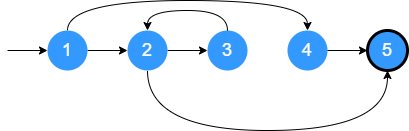
\includegraphics[width=8cm]{midterm-makeup-cfg1}
	\end{figure}

	\begin{parts}

		\part[5] List 5 examples of test paths. If this is not possible, explain why.
		\answerspace{20}
		\answer{}

		\part[5] State how many test paths there are in this CFG. Explain.
		\answerspace{10}
		\answer{Infinite.}

		\newpage
		\part[8] List all simple paths.
		\answerspace{25}
		\answer{
			[1, 2]
			[1, 4]
			[2, 3]
			[2, 5]
			[3, 2]
			[4, 5]
			[1, 2, 3]
			[1, 2, 5]
			[1, 4, 5]
			[2, 3, 2]
			[3, 2, 5]
			[3, 2, 3]
		}

		\part[6] List all prime paths.
		\answerspace{25}
		\answer{
			[1, 2, 3]
			[1, 2, 5]
			[1, 4, 5]
			[2, 3, 2]
			[3, 2, 5]
			[3, 2, 3]
		}

	\end{parts}


	\newpage
	\question Consider the following control-flow graph. The labels indicate that the variable X is \textit{defined} in nodes 1 and 3 and \textit{used} in nodes 2 and 5.

	\begin{figure}[ht]
		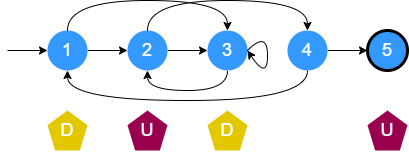
\includegraphics[width=8cm]{midterm-makeup-cfg2}
	\end{figure}

	\begin{parts}
	\part[4] List the test requirement set of all-defs coverage with respect to X.
	\answerspace{12}
	\answer{}

	\part[4] List the test requirement set of all-uses coverage with respect to X.
	\answerspace{12}
	\answer{}

	\part[4] List the test requirement set of all-du-paths coverage with respect to X.
	\answerspace{12}
	\answer{}

	\end{parts}





\if 0 %%%%%%%%%%%%%%%%%%%%%%%%%%%%%%%%%%%%%%%%%
	\question[10]
	\answerspace{30}
	\answer{}

	\question
	\begin{parts}
		\part[6]
		\answerspace{20}
		\answer{}

		\part[2]
		\answerspace{10}
		\answer{}

	\end{parts}
\fi %%%%%%%%%%%%%%%%%%%%%%%%%%%%%%%%%%%%%%%%%

	\newpage
	\begin{center}
		[EMPTY PAGE 1]
	\end{center}

	\newpage
	\begin{center}
		[EMPTY PAGE 2]
	\end{center}

\end{questions}


% 	\if 0
%
% 		\part[2] The \texttt{POPA} assembly instruction is a short form of the instruction \texttt{POP EAX}.
% 		\truefalse
% 		\answer{False. It POPS several registers.}
%
% 		\part[2] The Xinu \texttt{freemem} system call can coalesce the released block of memory with at most
% 		one other memory block from the free block list.
% 		\truefalse
% 		\answer{False. It can coalesce with two other blocks (optional: the block preceding it and the block succeeding it)}
%
% 		\part[2] Every semaphore initialized to one is a binary semaphore.
% 		\truefalse
% 		\answer{False. Semaphores initialized to one may still have values that go beyond one.}
%
% 		\part[2] The device driver is part of the operating system, not the hardware device.
% 		\truefalse
% 		\answer{True.}
%
% 		\part[2] The Xinu function calling convention passes arguments and return values on the stack.
% 		\truefalse
% 		\answer{False. Passes return values on a register (optional: EAX register).}
%
% 		\part[2] General-purpose OSs (e.g., Linux) allow user-mode code to change the contents of the interrupt vector.
% 		\truefalse
% 		\answer{False. To guarantee integrity and security only the OS is allowed to change the interrupt vector.}
%
% 		\part[2] An \texttt{\#ifndef} in the source code always causes the compiler to emit one or more machine instructions.
% 		\truefalse
% 		\answer{False. \texttt{\#ifndef} is preprocessor directive that does not emit instructions.}
%
% 		\part[2] The access time for CPU registers is shorter than for the CPU memory cache (e.g., L1).
% 		\truefalse
% 		\answer{True.}
%
% 		\part[2] The stack grows upwards in the x86 architecture.
% 		\truefalse
% 		\answer{False. It grows downwards.}
% 	\fi


	%=======================
%	\newpage
%
%	\question Static local variables can be accesses by more than one invocation of the function that declares it.
%	\begin{parts}
%		\part[4] Explain how can compilers support static local variables.
%		\answerspace{8}
%		\answer{They are store in the data/bss sections and used similarly to global variables so that their lifetime is the entire program run.}
%
%		\part[4] Do accesses to stack local variables need to be coordinated in a single-threaded application? Explain.
%		\answerspace{8}
%		\answer{No. Static local variable can only be accessed by one thread in a single-threaded application (i.e. no concurrency). [optional: signals]}
%
%		\part[4] Do accesses to stack local variables need to be coordinated in a multi-threaded application? Explain.
%		\answerspace{8}
%		\answer{Yes. Multiple threads may concurrently access the same object.}
%
%	\end{parts}
%
%
%
%	\question[10] Preemptive schedulers use a timer interrupt to call the scheduler every Q periods of time (quantum). In the context of
%	a preemptive round-robin scheduler, identify and explain three advantages of using long quantums over short quantums.
%	\answerspace{30}
%	\answer{Less CPU wasted on context switches, higher spatial / temporal locality}
%
%
%	%
%	\newpage
%	\question Consider the following graph which represents the concurrent execution of process P1 and process P2.
%	The Y and X axis represent the progress of process P1 and P2, respectively, and each point in the graph represents
%	a state of the system composed by process P1 and P2. Each of these processes needs to acquire, with exclusive access,
%	the shared resources R1 and R2 during their execution as represented in the diagram.
%
%	\begin{figure}[H]
%	\centering
%	\includegraphics[width=0.5\textwidth]{diagram-concurrency-crop}
%	\end{figure}
%
%	\begin{parts}
%		\part[4] Describe the situation represented by point C?
%		\answerspace{10}
%		\answer{Deadlock: P1 holds R1, P2 holds R2, P1 is blocked on R2, and P2 is blocked on R1.}
%
%		\part[4] Describe the situation represented by zone B?
%		\answerspace{10}
%		\answer{Impossible executions where both processes hold R1 and R2.}
%
%		\part[4] Describe the situation represented by zone A?
%		\answerspace{10}
%		\answer{Both processes already hold one of the resources and a deadlock will occur.}
%	\end{parts}
%
%
%
%	\newpage
%	\question[6] Describe and explain two differences between function calls and system calls. Describe which hardware mechanism(s) can be leveraged to implement system calls
%	in the context of general-purpose (secure) operating systems such as Linux.
%	\answerspace{20}
%	\answer{Function calls: call routines inside the program, fast. System calls: call
%	operating system services, slow. System calls can be implemented with software interrupts
%	and other specialized CPU instructions (optional: \texttt{syscall}/\texttt{sysenter}).}
%
%	\question[5] The \texttt{select} system call can be used in Linux in the context of files and sockets.
%	Explain the purpose of this system call and how applications can use it.
%	\answer{\texttt{select} receives a set of file descriptors and/or a timeout. The system call returns
%	when the file descriptors are ready to perform certain operations (e.g read/write). \texttt{select} is often used
%	in event-driven programs or when the program has to simultaneously operate on several file descriptors.}
%	\answerspace{5}
%
%
%	\newpage
%	\question
%	Consider the following coding problem that simulates a hospital.
%	The hospital classifies patients into two categories: Critical (C) and Minor (M). Each patient is modeled as
%	a thread that executes the function \texttt{void patient(bool is\_critical)}.
%	You can assume that synchronization primitives implement a FIFO policy.
%	All patients wait in a single line and are treated according to the following rules:
%
%	\begin{itemize}
%		\item All Critical patients must be treated before Minor patients
%		\item The order within patients of the same category must be maintained.
%		\item Doctors must finish treating their current patient before treating the next patient and no patient should be waiting in line if there is a free doctor.
%	\end{itemize}
%
%	\begin{parts}
%	\vspace{0.5 cm}
%		\part[10] Solve the problem described above using conditinal variables by assuming that there is only one doctor.
%		Model the doctor by making the patient thread sleep for an unknown amount of time.
%
%		\newpage
%		\part[10] Consider the same problem but with the following additional requirement:
%		\textit{There are 10 doctors and all doctors are capable of treating patients in the Minor category.
%		However, only some of those doctors (i.e., super doctors) are capable of treating patients in
%		Critical category.} Solve this problem using conditional variables.
%		Model each doctor as another thread and each doctor thread execute the function \texttt{void doctor(bool is\_super)}.
%
%
%	\end{parts}
%
%
%
%	\newpage
%	\question[15]
%	Consider the following coding problem that simulates a chemical reaction. Each thread will model an individual atom that enters a reaction chamber. An atom announces its presence by calling the appropriate \texttt{*\_available()} function for its type.
%	You can assume that synchronization primitives implement a FIFO policy.
%	These functions should implement the following functionality, making sure that the system makes progress whenever it is possible to do so:
%	\begin{itemize}
%		\item The \texttt{*\_available()} function should not return to its caller until a successful reaction has taken place.
%		\item The reaction chamber is very small. So, while a carbon or oxygen atom is in the reaction chamber, all other available carbon and oxygen atoms should wait.
%		\item Hydrogen molecules will preferentially react with a carbon atom if carbon is present, or an oxygen atom if a carbon atom is not available but oxygen is. Any number of hydrogen atoms can enter the reaction chamber.
%		\item Only two reactions are possible: 4 hydrogen atoms (H) can react with a carbon atom (C) to form methane, or 2 hydrogen atoms (H) can react with an oxygen atom to form water. Once the reaction chamber contains sufficient atoms of the right kind for a reaction to take place, all atoms involved in that reaction, [4H + 1C] in the former case and [2H + 1O] in the latter case, should leave the reaction chamber.
%	\end{itemize}
%
%	Solve this problem using \textbf{conditional variables} by implementing the \texttt{hydrogen\_available()}, \\
%	\texttt{carbon\_available()}, and \texttt{oxigen\_available()} functions.
%
%	% \question[10] Some operating systems support loadable kernel modules. Explain how you would implement kernel modules in Xinu.
%	% \answerspace{40}
%	% \answer{}
%
%
%	\newpage
%	\bonusquestion[6] Xinu currently runs on a single CPU. Explain how this affects the design of Xinu and how you
%	would modify Xinu to make it support more than one CPU.
%	\answerspace{40}
%	\answer{Xinu currently only needs to coordinate with the interrupt handlers and relies for this on interrupt disabling. Multi-core
%	support would require changing this either by using a single kernel lock (easy to implement but slow) or using finer-granularity
%	synchronization. The scheduler would need to be modified as well (e.g., several running processes, several null processes, etc.).}
%
%	\bonusquestion[4] Explain why an operating system can save less state of the running process on a system call
%	than on a hardware interrupt. Explain which state needs to be saved in each of these two contexts.
%	\answer{State saved for interrupts: all program state; for system calls: only what is required by the calling convention.
%	All state needs to be saved on interrupts because the process has no control over when they happen.}
%	\newpage
%
%



\end{document}
